% !TEX root = ../arbeit.tex
\chapter{Hardware Implementation}

Several \acf{PROCAMS} hardware designs have been proposed but often they are bulky, very expensive or need additional environmental instrumentation.
To fulfil the gathered requirements from~\autoref{chapter:requirements} several technologies are evaluated. Focus of attention is on size and quality on the one hand but also the price on the other.
To equip homes with multiple PROCAMSs they need to be affordable.

\section{Actuator}\label{actuator}
Actuators are necessary in order to realise the movement of the \ac{PROCAMS} as well as the automatic focus. There are basically two kinds of electric motors which suit the requirements: stepper motors and servos. 

A stepper motor is a synchronous brushless electric motor.
Rotations are divided into 200 to 400 equal steps. To control the motor, a micro-controller and a additional motor driver is needed. The motor can move step by step or hold the current position. There is no feedback about the current position since the stepper motor has no sensors. For a closed-loop control of the pan-tilt unit, separate sensors are needed, for example an accelerometer and a compass.
Otherwise, the system has to execute a self-calibration each launch to determine the movement constraints and the mapping between steps and position. 

In contrast to a stepper motor, a servo is a combination of an electro motor and a sensor, which provides position and speed feedback.
The position is controlled by a \ac{PWM} signal which can be generated by a micro-controller. The output shaft is moved depending on the difference between the commanded position and the measured position. The position is typically determined by a potentiometer. This allow up to 36000 steps per rotation. Servos are generally used in small robotics. Besides servos for rotational movement, there are also linear moving servos. 

Servo motors with high quality potentiometer offer up to 36000 possible positions per rotation compared to 400 of a stepper motor. Power is only consumed as the servo rotates. A stepper motor continues to consume power while holding a commanded position. As consequence, it runs warm. Finally, stepper motors need additional hardware to control precise positioning. Considering these arguments, using servos as actuators seems to be the superior approach. 

\section{Microcontroller}
A separate microcontroller is needed to command the actuators. When using a servo the microcontroller outputs a \ac{PWM} to set the position of the servo. Using a stepper motor, the microcontroller commands the number of steps to the motor driver.  

A wide variety of microcontrollers which can be used as a servo or stepper motor controller are available. However, embedded programming and an external programmer are necessary. 
The USB IO Board from Hardkernel\footnote{\url{http://www.hardkernel.com/main/products/prdt_info.php?g_code=G135390529643} visited: 02.04.14} allows easy upgrading of the firmware via USB. It provides a PWM interface via a \ac{PIC} microcontroller. Nevertheless, low level programming is required. 

Boards like the IOIO-OTG\footnote{\url{http://ytai-mer.blogspot.de/2013/01/go-go-ioio-on-go.html} visited: 02.04.14}, mainly developed by Ytai Ben-Tsvi, provide similar interfaces. The IOIO-OTG is especially designed to work with Android devices. A Java based API offers abstract and lucid programming. With such a board and the provided API neither low level programming nor an external programmer is necessary. 

Another platform offering effortless microcontroller programming is Arduino \cite{Arduino:b6u8ceDY}. It is an open-source prototyping platform combining software and hardware. Many boards in different sizes and versions are available to suit different use-cases. Whereas, hardware design is open-source there are also less expensive boards from third-party manufacturers obtainable. The microcontroller is programmed with a platform independent IDE based on the Processing IDE. Various Arduino libraries are linked to simplify C and C++ programming. The servo library for example, allows setting the position of the servo with one simple command. Regarding these arguments, Arduino is used as microcontroller platform. 

\section{Projector}
Projection technologies became more sophisticated over the years. New technologies allow smaller and less power consuming devices. Projectors can be classified by light source and projection technology. Typically light sources are laser, LED, arc lamps and combinations of laser and LED. Arc lamps consume much power and become very hot. So, they require a powerful cooling system which makes them loud and bulky. Therefor, projectors with an arc lamp are not further examined.

There are three major projection technologies utilising lasers as light source \cite{Mertens:p40QFV-L}. With Laser-Beam-Steering the image is created pixel by pixel by a laser beam guided across the projection surface by using a mirror. Combining three lasers with different colours (red, green, blue) and intensity using optics, a full coloured image is created. Light Blue Optics \cite{Blue:2014ab} developed Holographic Laser Projection where a laser illuminates a hologram that diffracts the laser to create the original image. Light Blue Optics claim, that it is very power efficient and has less speckle than other laser projector technologies. A new technology combines lasers and \ac{LCoS} to project an image. White laser light as a combination of red, blue and green is used to illuminate the \ac{LCoS}, which control the amount of reflected light by changing polarisation. Research showed \cite{Guttag:2011wd} that with this approach more eye safety, lower power consumption and higher resolution are possible. All three technologies using laser light have the advantage that the image is always in focus. No manual refocusing is necessary. However, maximum brightness of laser projectors is 50 ANSI Lumen which requires a dimmed environment for acceptable visibility. 

One of the most mature technologies using LEDs as light source is \ac{DLP} developed by Texas Instruments \cite{Rukzio:2012hj}.
Light is emitted to tiny mirrors on a chip that directs the light. Dependent on the state, light is reflected to the surface or an absorber. Colour is generated by a rotating colour wheel splitting the light into red, blue and green. The above described technology using \ac{LCoS} is also used with LEDs, but this time focusing optics are necessary. Since LEDs are not getting very hot while operating, small and energy efficient projectors with LEDs are available. While maximal brightness of tiny laser projectors is limited to 50 Lumen, LEDs projectors provide up to 550 lumen without exceeding the size of half cubic decimetre.

\section{Depth Sensing Camera}\label{sec:depthsensingcamera}
Three distinct technologies are applicable to generate depth information~\cite{Ko:2012vp}. Stereoscopic vision systems use two slightly offset cameras and compare the obtained images. On basis of the difference in location of a point in corresponding images, the depth can be calculated. Stereoscopic vision systems are very low-cost but high in software complexity. The depth accuracy is only in the cm range. 

Depth sensing cameras using \ac{SL} pattern have also high software complexity but offer, dependent on the model, depth accuracy in \textmu m to cm range. In comparisons to a stereoscopic vision system, one camera is replaced by a laser or led light source which creates a light pattern. This pattern is obtained by the remaining camera. To acquire depth information the same technique is used, but due to the pattern, finding corresponding points is easier and more accurate.

A relatively new technology is \ac{ToF}. It allows depth accuracy in the mm range. An emitter transmits a light pulse to an object. There it gets reflected and finally determined again by the receiver. The distance of an object can be calculated by measuring the time between transmit and receive of the light pulse. Available \ac{ToF} cameras have only a quarter of pixel resolution compared to \ac{SL} cameras. But temporal resolution with up to 160 \ac{fps} (Argos 3D - P100) is very high.

\begin{table}[htb]
\begin{tabularx}{\textwidth}{ l X l l p{1.9cm} p{1.9cm}}
\toprule
Type & Tech-nology & Range (m) & FOV (H,V) & Depth res. (w x h,fps) & Colour res. (w x h,fps) \\
\midrule
Kinect XBOX & SL & 0.8 - 10.0 & 57.0, 43.0 & 640x480,30 & 1280x960,12 \\
Kinect Windows & SL & 0.4 - 3.0 & 57.0, 43.0 & 640x480,30 & 1280x960,12 \\
Kinect 2 & ToF & 0.8 - 4.0 & 70.0, 60.0 & 512x424,30 & 1920x1080,30 \\
Carmine 1.08 & SL & 0.8 - 3.5 & 57.5, 45.0 & 640x480,60 & 640x480,60 \\
Carmine 1.09 & SL & 0.35 - 1.4 & 57.5, 45.0 & 640x480,60 & 640x480,60 \\
DS311 short & ToF & 0.15 - 1.0 & 57.3, 42.0 & 160x120,60 & 640x480 \\
DS311 long & ToF & 1.5 - 4.5 & 57.3, 42.0 & 160x120,60 & 640x480 \\
DS325 & ToF & 0.15 - 1.0 & 74.0, 58.0 & 320x240,60 & 1280x720 \\
Senz3D & ToF & 0.15 - 1.0 & 74.0, 58.0 & 320x240,30 & 1280x720 \\
\bottomrule
\end{tabularx}
\caption{Depth sensing camera overview.}
\label{tab:cams}
\end{table}
In~\autoref{tab:cams} a brief overview of several commercially available depth sensing cameras is given. 
In late 2013, Apple bought PrimeSense the manufacturer of the Carmine cameras. Ever since PrimeSense cameras are no longer available for purchase.
The DepthSense311 (DS311) and DS325 are developed by SoftKinetic a Belgian company. The Kinect and Kinect 2 is manufactured by Microsoft, but by now it is not possible to develop applications with the Kinect 2. Senz3D bases on the DepthSense311 and is made available by Creative.
	


\subsection*{SDKs and Frameworks}\label{sec:depthSDK}
Hardware manufacturers distribute powerful SDKs to minimise the challenges in developing frameworks or applications which their depth sensing cameras. Moreover, there is a big community developing frameworks, offering numerous useful functionalities and services.

The Kinect SDK is used to develop Kinect-enabled applications. It includes Kinect Fusion and  Kinect Interactions. With Kinect Fusion it is possible to create a 3D reconstruction of objects or the environment in real time. Kinect Interaction provides gesture recognition. iisu, an acronym for ''The Interface Is You``, is the 3D gesture recognition development framework by SoftKinetic. As well as Kinect SDK it supports full body tracking and natural gesture development and recognition. Intel Perceptual Computing SDK supports body and gesture recognition as well as facial analysis, hand and finger tracking. The SDK focuses on short range interaction in particular. \ac{OpenNI} is an open source SDK for middleware and application development mainly driven by PrimeSense. The framework supports voice and voice command recognition, hand gestures and full body motion tracking. The point cloud library (PCL) is an open source library which offers many algorithms for n-dimensional point could processing. In the context of depth sensing, the provided algorithms like filtering, surface reconstruction, or segmentation allow sophisticated analysis of the scenery.~\autoref{tab:depthFrameworks} summarises which depth sensing camera receives the support of which framework.
\begin{table}[htb]
\vspace{4em}
\centering
\begin{tabular}{r|ccccc} &
\begin{rotate}{60} OpenNI \end{rotate} &
\begin{rotate}{60} Kinect SDK  \end{rotate} &
\begin{rotate}{60} Intel PC SDK  \end{rotate} &
\begin{rotate}{60} IISU  \end{rotate} &
\begin{rotate}{60} PCL \end{rotate} \\ \hline
Kinect        & \CIRCLE  &   \CIRCLE 	 &  \Circle    	& \CIRCLE    & \CIRCLE  \\
Kinect 2        & \Circle      &   \LEFTcircle  &  \Circle    	& \Circle       & \Circle  \\
Carmine        & \CIRCLE  &   \Circle   	 &  \CIRCLE  	& \CIRCLE   &  \CIRCLE\\ 
DepthSense  & \Circle     &   \Circle   	 &  \CIRCLE  	&\CIRCLE   &\Circle \\ 
Senz3D	     & \CIRCLE  & \Circle  		&  \CIRCLE	& \CIRCLE  & \CIRCLE	\\
\hline
\end{tabular}
\caption{Overview of supported SDKs. \\\CIRCLE supported  \Circle not supported  \LEFTcircle announced}
\label{tab:depthFrameworks}
\end{table}



\section{Single Board Computer}\label{sec:sbc}
The hardware design of the proposed stand-alone PROCAMS includes a processing unit which is fixed near to the projector and camera. The processing unit needs to be small and lightweight. To connect WiFi, microcontroller and the depth sensing camera, at least three USB-ports are mandatory. These requirements lead to a so called \ac{SBC}, a complete computer built on a single circuit board. To handle all computations a high performance SBC is essential. An overview of currently existing SBC is given in~\autoref{tab:sbc}.
It should be noted that most of the high performance SBC utilise the ARM \ac{ISA}. Deduced from mobile phone processors, SBC processors are very energy efficient, produce little heat and have similar computational power as present mobile phones. 
However, using the ARM architecture narrows the choice of \acfp{OS} to Linux and Android.

\begin{table}[htb]
\begin{tabularx}{\textwidth}{ l l X l X l l}
\toprule
NAME & CPU (GHz) & RAM (MB) & USB & SIZE (cm) & \acs{ISA} & \acs{OS} \\
\midrule
 ODROID-XU & 4x(1.6 + 1.2) & 2048 & 4/2 & 7x9.4 & ARM & L, A \\
 ODROID-X2  & 4x1.7 & 2048 & 6 & 9x9.4 & ARM & L, A \\
 ODROID-U2 & 4x1.7 & 2048 & 2 & 4.8x5.2 & ARM & L, A \\
 Origen Board & 4x1.4 & 1024 & 2 & 11.9x11.9 & ARM & L, A \\
 Arndale Board & 2x1.7 & 1024 & 3 & 36x24 & ARM & L, A \\
 Nitrogen6X & 4x1 & 1024 & 2 & 11.4x7.6 & ARM & L, A, W-CE \\
 Sabre Lite  & 4x1 & 1024 & 2 & 8.25x8.25 & ARM & L, A, W-CE \\
 Via Epia-P910 & 4x1 & 512 & 2 & 10x7.2 & X86 & W, X, L, A \\
\bottomrule
\end{tabularx}

\caption{Single-board computer overview. Operating system acronyms: \textbf{L}inux, \textbf{A}ndroid, OS \textbf{X}, \textbf{W}indows and  \textbf{W}indows-\textbf{CE}}
\label{tab:sbc}
\end{table}

\section{Used Hardware}
\paragraph{Actuator}
For pan and tilt of the PROCAMS two HS-785HB by HiTEC are used. This are quarter scale servos with a torque of \SI{132}{\N\cm} at \SI{6}{\volt}. They are one of the stronger servos in this size segment. Based on the data sheet, a full rotation takes less than \SI{9}{\second}.
Focus is driven by a NYA 2.9g linear long throw servo SPMSH2040L from Spektrum with a torque of 329g running at \SI{4.2}{\volt}.

\paragraph{Microcontroller}
Actuators are controlled by an Arduino Pro Mini. This is one of the smallest Arduino boards. It is built on the ATmega168 with six PWM output pins for servo control. Arduino is used because it offers great library support for servo control as well es easy prototyping. 

\paragraph{Projector}
For the proposed PROCAMS the ultra-compact LED projector ML550 by OPTOMA is used. In this projector, DLP technology by Texas Instruments combined with a LED light source is deployed. It measures only \SI{105 x 106 x 39}{\mm} in size and weights \SI{380}{\g}. The projection distance is between \SI{0.55}{\meter} and \SI{3.23}{\meter}.

\paragraph{Depth Sensing Camera}
The depth sensing cameras presented in~\autoref{sec:depthsensingcamera} can be divided into short (less than 1.4 metres) and long distance sensing cameras. Derived from the interviews, a long distance sensing camera is necessary. For deployment, the Carmine 1.08 from PrimeSense was chosen. It has a smaller form factor than the Kinect and a higher depth resolution than the DS311. Moreover, it is supported by all presented Frameworks except the Kinect SDK.  

\paragraph{Single Board Computer}
As processing unit, the ODROID-XU was chosen. It is developed by Hardkernel a South Korean open source hardware company. ODROID-XU is one of the most powerful SBC available. The CPU is based on big.LITTLE architecture which features a powerful eight-core for efficient handling of multitasking. Besides it has enough ports to connect the Android Pro Mini microcontroller, the depth sensing camera as well as a WiFi-Dongle and keyboard. 


\section{Pan-Tilt Unit}
The pan-tilt unit is responsible for moving the complete PROCAMS, in detail the depth sensing camera, the projector and the SBC. 
There are commercially available pan-tilt units e.g. the D46-17build by FLIR or the MPT1100-SS retailed by ServoCity. However, these products are heavy, large in size and expensive. Prises are around 650 to 2500 USD. Tending to an affordable lightweight stand-alone \ac{PROCAMS}, an approach with servo motors looks promising. A direct drive mechanism without any reductions minimises additional gearing and bearing parts.

\pagebreak
Each of the tilt and pan servo is grounded to a \textit{ServoBlocks} by ServoCity. A ServoBlocks isolates the lateral load from the servo and increase the load-bearing. ServoBlocks are easily screwed together to create rigid structures actuated by servos.  An image of a servo fixed to a \textit{ServoBlocks} is illustrated in~\autoref{img:servo}.

\TwoFig{images/hardware/servo.jpg}      {ServoBlocks construction}                  {img:servo}
       {images/hardware/pantilt.png}{Pan-Tilt unit}{img:pantilt} {Hardwar and construction of pan-tilt unit} {}
       
The pan servo is mounted overhead. To gain more open space for tilting, a 3D-printed \ac{PLA} spacer (see~\autoref{img:spacer}) is connected to the hub shaft. The tilt servos is rotated by \SI{90}{\degree} in a vertical plane. The hub shaft is bolted to the other side of the spacer. A complete illustration of the pan-tilt unit is shown in~\autoref{img:pantilt}.
\begin{table}[htb]
\begin{tabularx}{\textwidth}{ X p{2cm} X l}
\toprule
Command  & Code & Value & Description \\
\midrule
Position & 00 & - & Returns pan and tilt value \\
Pan & 01 & Position in \textmu s & Pan to given position \\
Tilt & 02 & Position in \textmu s & Tilt to given position \\
Focus & 03 & Position in \textmu s & Focus to given position \\
\midrule
Up & 04 & - & Moves unit up \\
Down & 06 & - & Moves unit down \\
Left & 05 & - & Moves unit left \\
Right & 07 & - & Moves unit right \\
\bottomrule
\end{tabularx}
\caption{Implemented commands for pan-tilt unit and focus control}
\label{tab:arduinoCommands}
\end{table}
\pagebreak
The servos are controlled by the previous presented Arduino Mini Pro. The Arduino framework provides a servo library which allows simple servo control. Via serial interface the ODROID-UX SBC can send commands to the Arduino board which are translated into servo control commands.  Commands are seperated into command code, and optional values. Code and values are separated by a \# character. The command to pan to a specific direction for example is:  \verb+pan#position+ respectively \verb+01#1580+ where position is the pulse width in \textmu s. All supported commands are summarised in~\autoref{tab:arduinoCommands}. 

\begin{figure}[htbp]
        \centering
        \begin{subfigure}[b]{0.3\textwidth}
                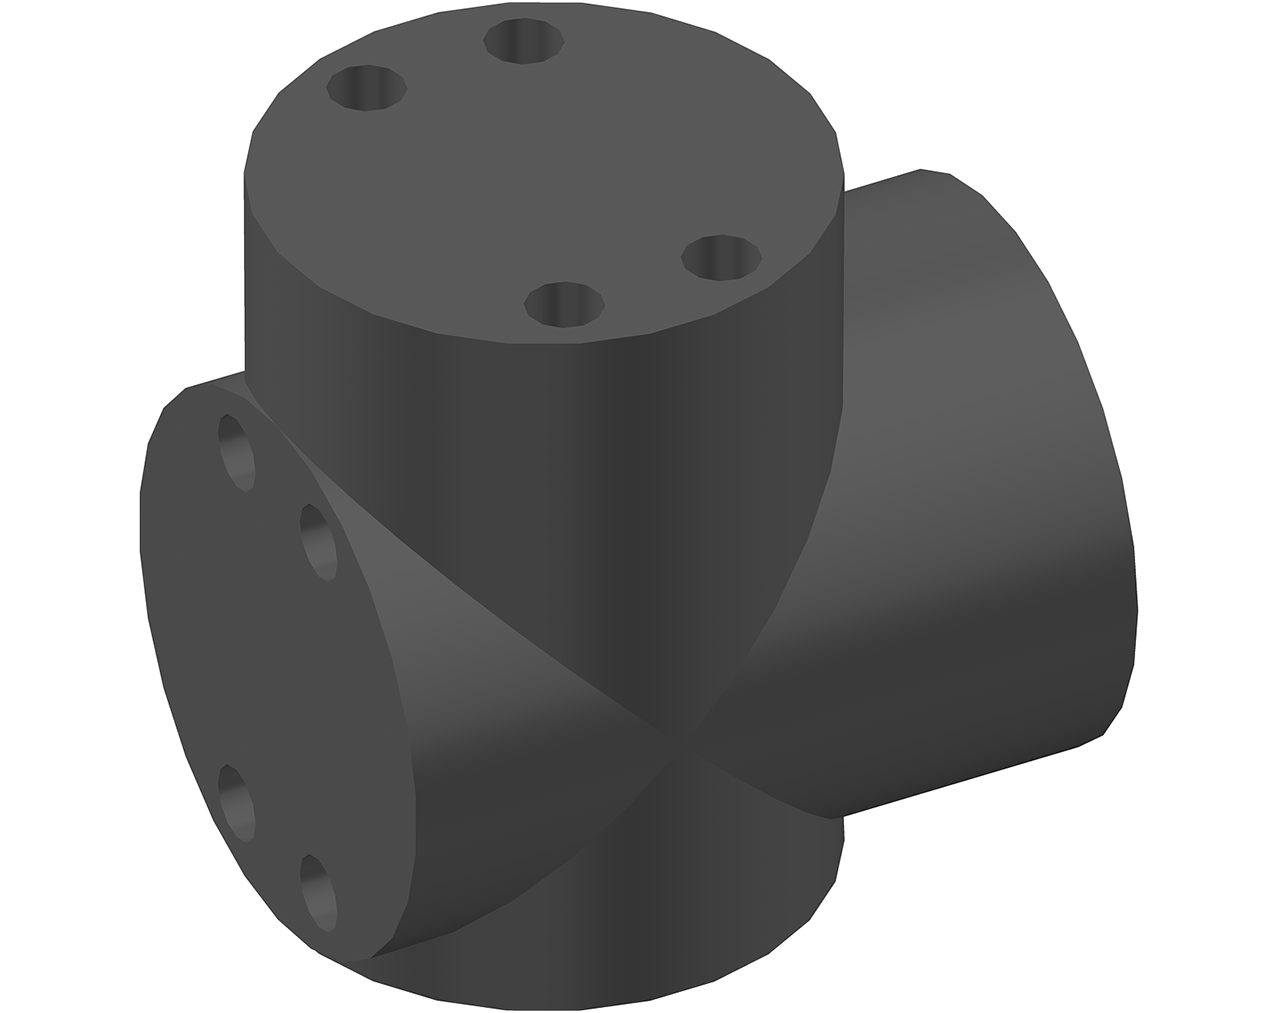
\includegraphics[width=\textwidth]{images/cad/spacer.png}
                \caption{Pan-Tilt unit spacer}
                \label{img:spacer}
        \end{subfigure}
        \quad
        \begin{subfigure}[b]{0.3\textwidth}
                \includegraphics[width=\textwidth]{images/cad/focus.png}
                \caption{Focus handle grabber}
                \label{img:focusHandle}
        \end{subfigure}
         \quad
         \begin{subfigure}[b]{0.3\textwidth}
                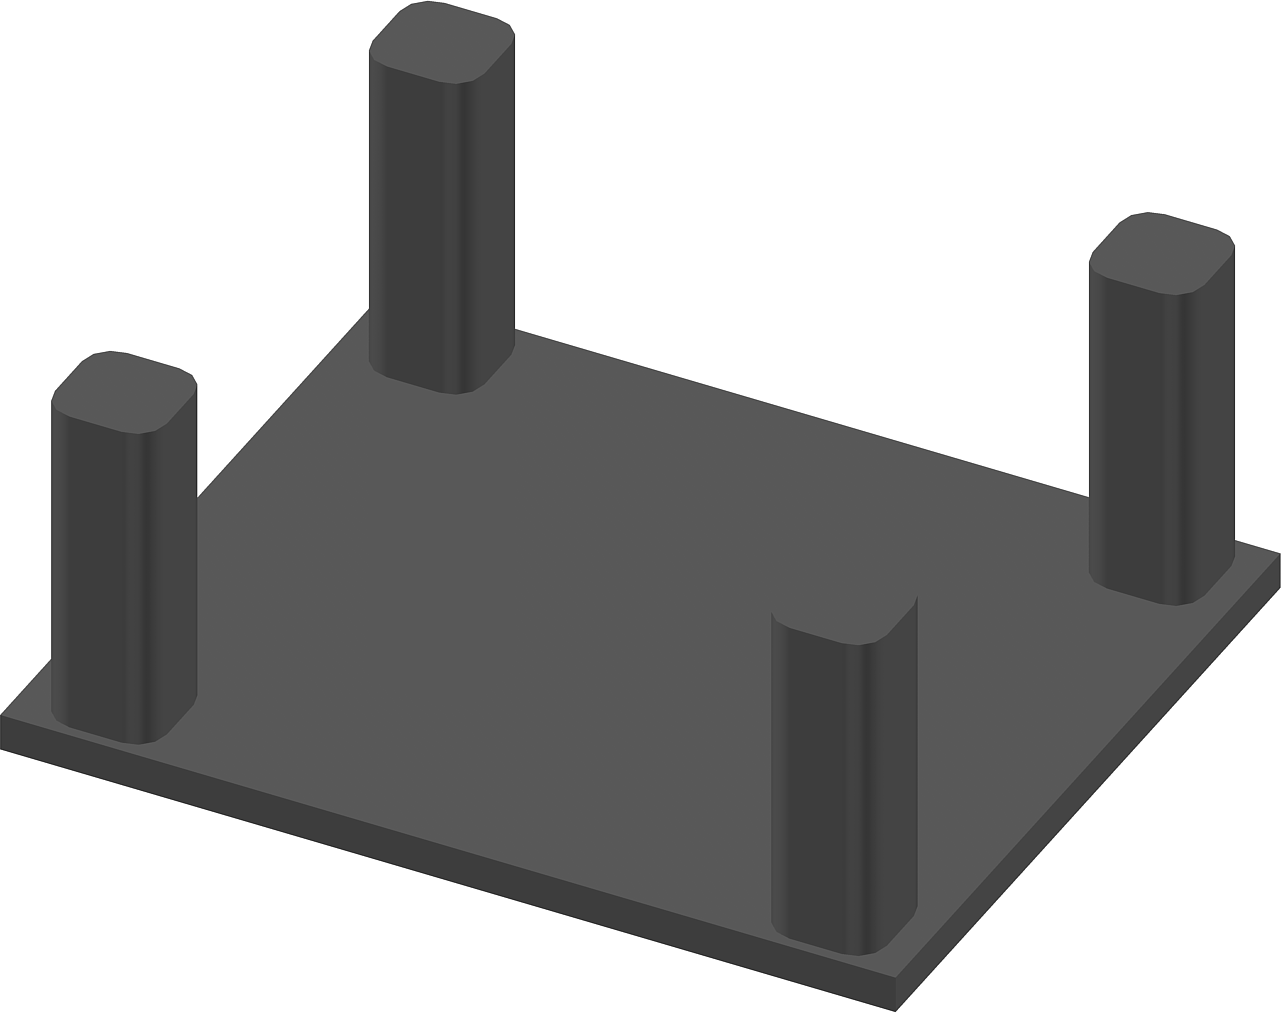
\includegraphics[width=\textwidth]{images/cad/servo.png}
                \caption{Focus servo mount}
                \label{fig:focusServo}
        \end{subfigure}
        \caption{3D-representations of the special designed parts}
\end{figure}

\section{Focus}
% !TEX root = ../arbeit.tex
\begin{wrapfigure}{r}{0.5\textwidth}
\vspace{-1em}
  \centering
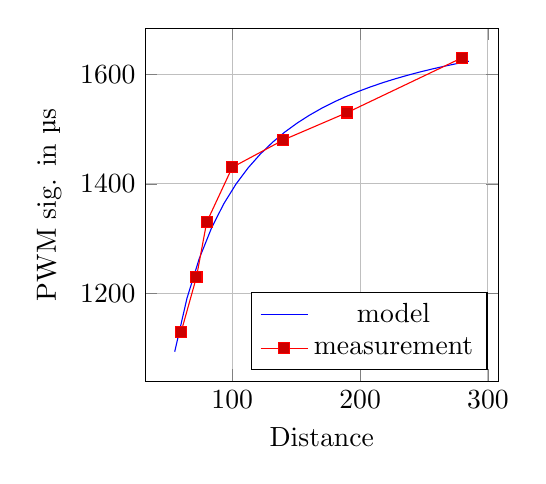
\begin{tikzpicture}
	\begin{axis}[
    /pgf/number format/.cd,
        1000 sep={},
        		height=.5\textwidth,
		width=.5\textwidth,
		grid=major,
		legend pos=south east,
		xlabel=Distance,
		ylabel=PWM sig. in \textmu s,
	]	
	\addplot[draw=blue][domain=55:285] {-36076/x + 1750};
	\addlegendentry{model}
	\addplot coordinates {
(60,1130)
(72,1230)
(80,1330)
(100,	1430)
(140,1480)
(190,1530)
(280,1630)};
	\addlegendentry{measurement}
	\end{axis}
	\end{tikzpicture}
         \caption{Focus-Distance model}

\label{plot:focus}
\end{wrapfigure}
The focus of the Optoma 550ML is manually adjusted via a small lever. To realise automatic adjustment of the focus, the movement of the lever must be controlled with a servo. A linear servo is used for this task. The servo is glued to the designed servo mount shown in~\autoref{fig:focusServo}. This construction is then glued to the projector, left of the adjustment lever. A special piece is designed (see~\autoref{img:focusHandle}) which grabs the lever and is also connected via a steel wire to the servo. The complete construction is illustrated in~\autoref{fig:autofocus}. The servo is controlled in the same way as pan and tilt servo.

To determine the required position of the servo for a given distance a calibration task was conducted. The projector was placed at seven different distances between \SI{0.6} and \SI{2.8}{\meter} perpendicular to a wall. The corresponding PWM signal that produces the visually sharpest focus was determined. These seven distance--PWM value pairs were used to determine the formula for setting the focus. Non-linear regression with two parameters was used for analysis.
Analysis leads to:
\begin{equation}
\nonumber
\notag
\mathit{PWM}=\frac{-36076.6267}{distance} + 1750.06825
\end{equation}
Where $\mathit{PWM}$ is the PWM signal in \textmu s and  $distance$  is the distance between surface and projector in cm. The measured values and the calculated formula are plotted in~\autoref{plot:focus}. Maximum error is less than 40\textmu s which does not lead to projections which are out of focus.

\begin{figure}[htbp]
        \centering
        \begin{subfigure}[b]{0.61\textwidth}
                \includegraphics[width=\textwidth]{images/hardware/focus.png}
          	\caption{Autofocus construction}
         	\label{fig:autofocus}
        \end{subfigure}
          \hfill
        \begin{subfigure}[b]{0.31\textwidth}
                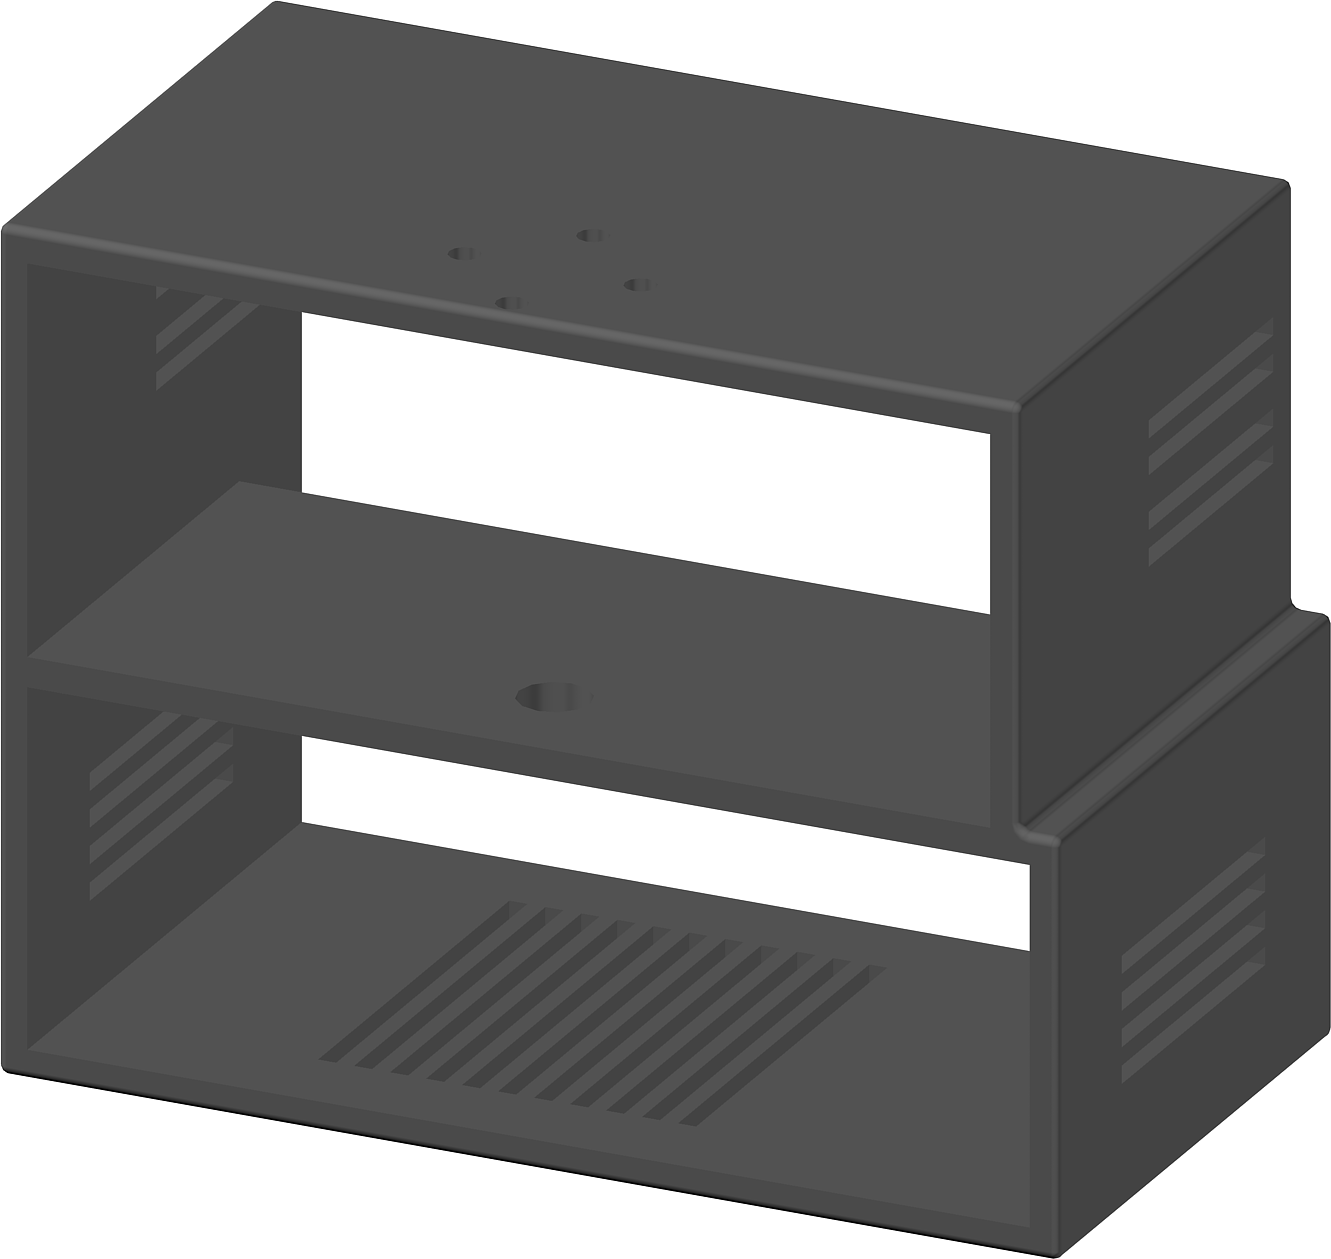
\includegraphics[width=\textwidth]{images/cad/case.png}
                \caption{Projector and SBC case}
                \label{img:projectorCase}
        \end{subfigure}
        \caption{Hardware construction}\label{img:cad}
\end{figure}
	
\section{Construction}
After assembling the pan-tilt unit and preparing the auto focus, the complete hardware of the PROCAMS is assembled and wired. To connect the projector and SBC with the pan-tilt unit a special case (see~\autoref{img:projectorCase}) is designed and 3D-printed. The PrimeSense depth sensing camera is glued to the bottom of the projector facing the same direction with a maximum overlap of both fields of views. The final hardware construction is illustrated in~\autoref{img:finalConstruction}. 

It measures only \SI{10.5 x 12.2 x 22.5}{\cm} including the pan-tilt unit and weights \SI{996}{\g}. With a size of \SI{10.5x12.2x9}{\cm} excluding the protrude part of the camera and a weight of about \SI{690}{\g} the PROCAS itself (excluding the pan-tilt unit) is notable smaller and lighter.
The complete hardware can be bought and assembled for less than 1000 USD, assuming mechanical skill and access to a 3D printer. 

\begin{sidewaysfigure}[h] 
\centering 
                \includegraphics[width=\textwidth]{images/hardware/constructionFull.png}
                \caption{Complete construction of the stand-alone PROCAMS}
                \label{img:finalConstruction}
\end{sidewaysfigure}